\documentclass[tikz,border=10pt]{standalone}
\begin{document}
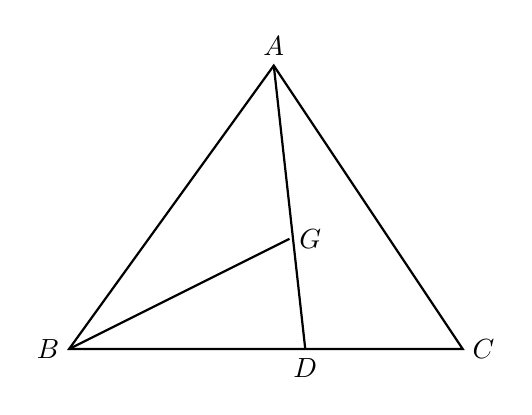
\begin{tikzpicture}
\coordinate (A) at (2.6,3.6);
\coordinate (B) at (0,0);
\coordinate (C) at (5,0);
\coordinate (D) at (3,0);
\coordinate (G) at (2.8,1.4);

\draw[thick] (A) -- (B) -- (C) -- cycle;
\draw[thick] (A) -- (D);
\draw[thick] (B) -- (G);

\node[above] at (A) {$A$};
\node[left] at (B) {$B$};
\node[right] at (C) {$C$};
\node[below] at (D) {$D$};
\node[right] at (G) {$G$};
\end{tikzpicture}
\end{document}
